%-------------------------------------------------------------------------------
%-------------------------------------------------------------------------------
%-------------------------------------------------------------------------------
\chapter{Affine par morceaux}
%-------------------------------------------------------------------------------
%-------------------------------------------------------------------------------
Il est usuel de chercher une droite de régression lorsqu'on a un tableau de données à deux dimension : $(x_i,y_i)_{1\le i\le n}$ avec $x_1< x_2 < \cdots < x_n$.

On cherche une droite d'équation $y= ax+b$ qui minimise l'erreur $\displaystyle e_{1,n}(a, b)=\sum_{i=1}^n \bigl(y_i-a x_i-b\bigr)^2$. 

On admettra que le temps de calcul de $e_{1,n}$ est linéaire en $n$.

Cependant parfois une série de données correspond à plusieurs réponses successives et il semble utile d'approcher ceux-ci par une fonction affine par morceaux.

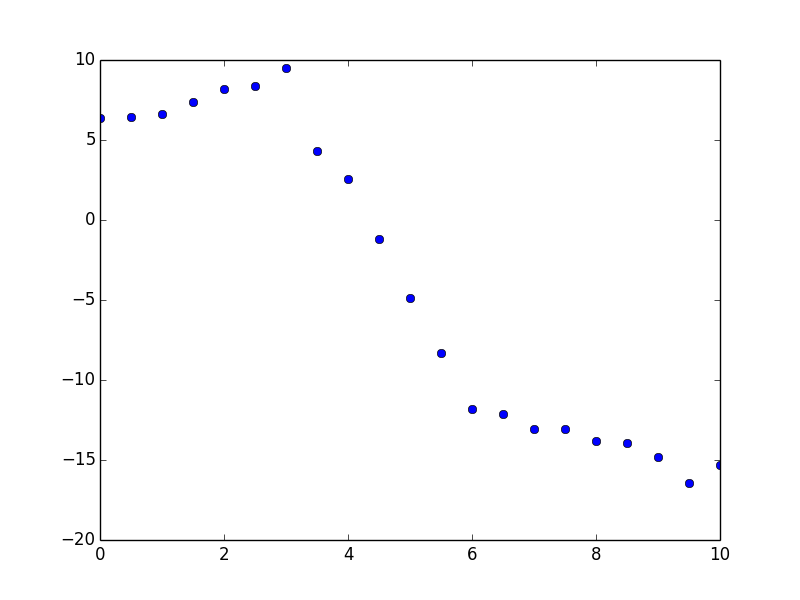
\includegraphics[width=8cm]{Oraux/Affine_1.png}
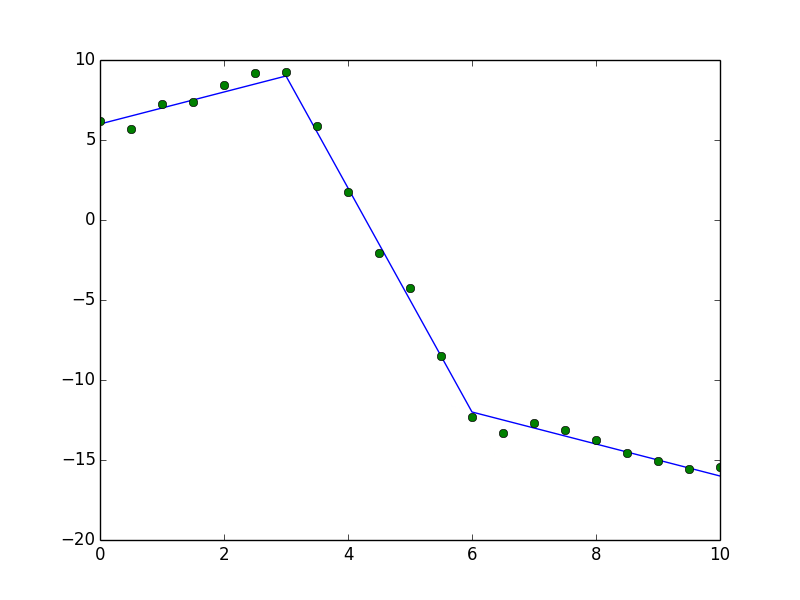
\includegraphics[width=8cm]{Oraux/Affine_2.png}

On note $\displaystyle e_{i, j}(a, b)=\sum_{k=i}^j \bigl(y_k-a x_k-b\bigr)^2$.

Un approximation affine par morceaux est définie par une suite $1=p_0 < p_1 < \cdots < p_m = n$
et des équations de droites $y = a_k x + b_k$ et son erreur est 
\[\sum_{k=1}^m e_{p_{k-1}, p_k} + (m-1) C\]
où $C$ est la pénalité d'un découpage.

Dans l'exemple ci-dessus la mesure de l'erreur est 
\[e_{1,7}(a_1, b_1)+e_{8,12}(a_2, b_2)+e_{13,21}(a_3, b_3) + 2 C\]

Proposer un algorithme de complexité polynomiale en $n$du calcul du minimum.
